% \section{Introduction}
\section{Introducción}

% ============================================================
% Initial GWAS explanation
% ============================================================
\begin{frame}{Estudios de Asociación Genómica (GWAS)}

  \centering
  \begin{minipage}[t]{0.48\textwidth}
    \centering
    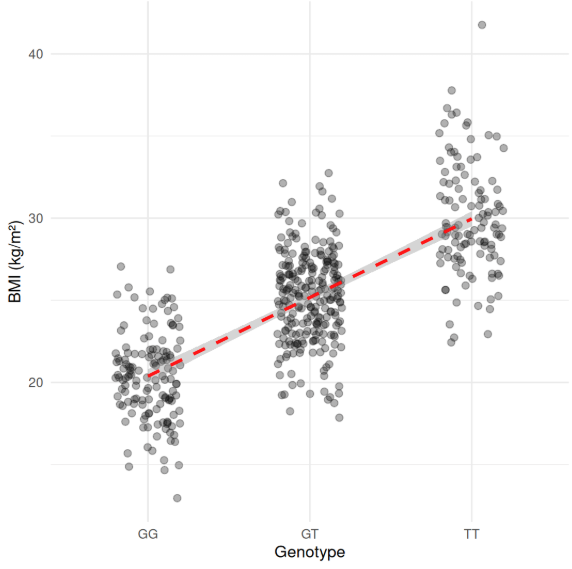
\includegraphics[width=\textwidth, height=5cm, keepaspectratio]{img/diagrams/single-locus.png}
    % \captionof{figure}{Single-variant linear model for simulated Body Mass Index (BMI) data.}
    \captionof{figure}{Modelo lineal de una sola variante con datos simulaods para Índice de Masa Corporal (BMI).}
  \end{minipage}
  \hfill
  \begin{minipage}[t]{0.48\textwidth}
    \centering
    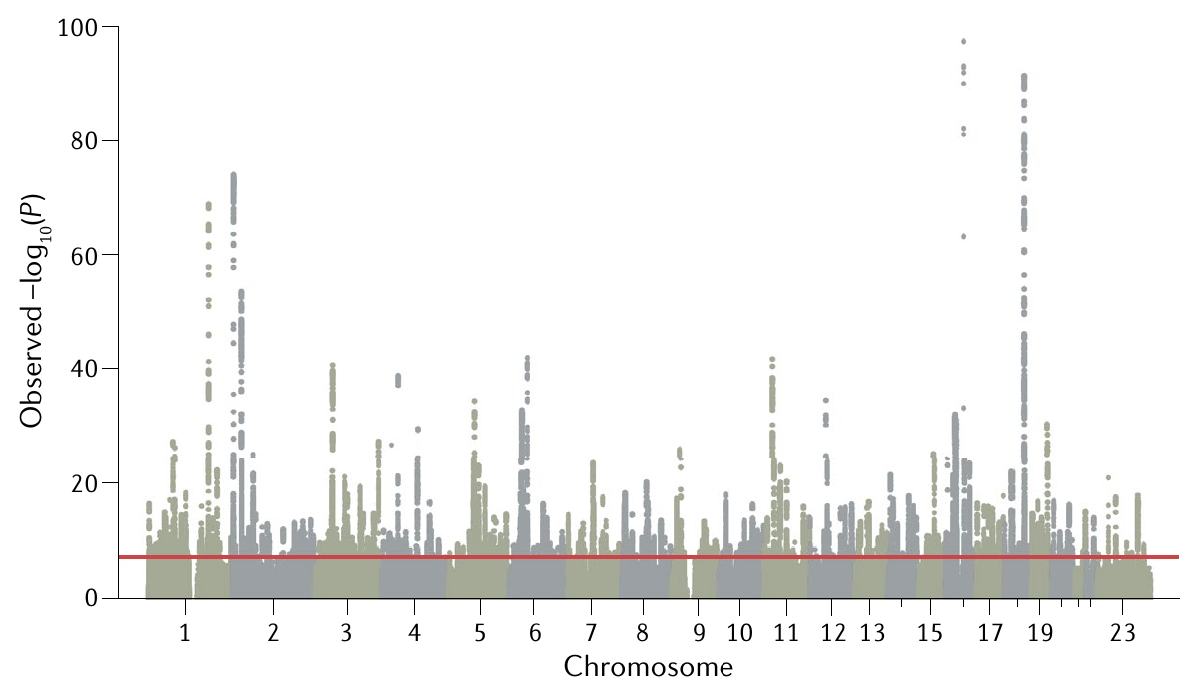
\includegraphics[width=\textwidth, height=5.5cm, keepaspectratio]{img/diagrams/manhattan.png}
    %\captionof{figure}{GWAS results showing the significance of each regression for Body Mass Index (BMI) (Uffelmann et al., 2021, Nature Methods Review).}
    \captionof{figure}{Manhattan Plot mostrando resultados de asociación de un GWAS para Índice de Masa Corporal (BMI) en una población europea. Recuperado de \parencite{uffelmann2021-gwas}.}
  \end{minipage}

\end{frame}

% ============================================================
% Animated TikZ: Genetic Effects Decomposition (two-column)
% ============================================================
\begin{frame}[b]{Sesgos en GWAS}

  \begin{columns}

    %% ---- LEFT COLUMN: stacked bar + legend ----
    \begin{column}{0.42\textwidth}
      \centering
      \begin{tikzpicture}[
        every node/.style={font=\sffamily},
      ]

        % --- Color definitions ---
        \definecolor{dgegray}{HTML}{3C3C3C}
        \definecolor{nurblue}{HTML}{1A7FA0}
        \definecolor{assred}{HTML}{7A1525}
        \definecolor{stratgray}{HTML}{B8B8B8}
        \definecolor{sideblack}{HTML}{1A1A1A}
        \definecolor{dimgray}{HTML}{D0D0D0}

        % --- Dimensions (narrower for column) ---
        \def\barW{2.4}
        \def\barX{0.7}
        \def\hdge{2.3}
        \def\hBlue{0.75}
        \def\hRed{0.6}
        \def\hGray{0.35}

        % --- Fixed bounding box (prevents bar from jumping between overlays) ---
        \useasboundingbox
          (\barX-0.8, -2.5) rectangle (\barX+\barW+0.1, \hdge+\hBlue+\hRed+\hGray+0.1);

        % --- Layer 1: dge (always visible) ---
        \fill[dgegray]
          (\barX, 0) rectangle (\barX+\barW, \hdge);

        % --- Layer 2: Crianza genética (overlay 2+) ---
        \only<2->{
          \fill[nurblue]
            (\barX, \hdge) rectangle (\barX+\barW, \hdge+\hBlue);
        }

        % --- Layer 3: Apareamiento selectivo (overlay 3+) ---
        \only<3->{
          \fill[assred]
            (\barX, \hdge+\hBlue) rectangle (\barX+\barW, \hdge+\hBlue+\hRed);
        }

        % --- Layer 4: Estratificación poblacional (overlay 4+) ---
        \only<4->{
          \fill[stratgray]
            (\barX, \hdge+\hBlue+\hRed) rectangle (\barX+\barW, \hdge+\hBlue+\hRed+\hGray);
        }

        % --- Sidebar: "Efectos de confusión" (overlay 2+) ---
        \only<2->{
          \fill[sideblack]
            (\barX-0.7, \hdge) rectangle (\barX, \hdge+\hBlue+\hRed+\hGray);
          \node[rotate=90, anchor=mid, text=white,
                font=\sffamily\bfseries\tiny]
            at (\barX-0.35, \hdge + 0.5*\hBlue + 0.5*\hRed + 0.5*\hGray)
            % {Confounding effects};
            {Efectos de confusión};
        }

        % --- Legend: order mirrors bar (top→bottom = Estrat, Apear, Crianza, dge) ---
        \def\legX{0.0}
        \def\legY{-0.5}
        \def\legSep{0.45}
        \def\legBoxW{0.25}
        \def\legBoxH{0.25}

        %% Row 0 (top): Estratificación — highlighted on overlay 4
        \only<4>{
          \fill[stratgray]
            (\legX, \legY) rectangle +(\legBoxW, -\legBoxH);
          \node[anchor=west, font=\sffamily\bfseries\scriptsize]
            at (\legX+\legBoxW+0.1, \legY-0.5*\legBoxH)
            % {Population Stratification};
            {Estratificación poblacional};
        }
        \only<1-3>{
          \fill[dimgray]
            (\legX, \legY) rectangle +(\legBoxW, -\legBoxH);
          \node[anchor=west, font=\sffamily\scriptsize, text=dimgray]
            at (\legX+\legBoxW+0.1, \legY-0.5*\legBoxH)
            % {Population Stratification};
            {Estratificación poblacional};
        }

        %% Row 1: Apareamiento selectivo — highlighted on overlay 3
        \only<3>{
          \fill[assred]
            (\legX, \legY-1*\legSep) rectangle +(\legBoxW, -\legBoxH);
          \node[anchor=west, font=\sffamily\bfseries\scriptsize, text=assred]
            at (\legX+\legBoxW+0.1, \legY-1*\legSep-0.5*\legBoxH)
            % {Assortative Mating};
            {Apareamiento selectivo};
        }
        \only<1-2,4>{
          \fill[dimgray]
            (\legX, \legY-1*\legSep) rectangle +(\legBoxW, -\legBoxH);
          \node[anchor=west, font=\sffamily\scriptsize, text=dimgray]
            at (\legX+\legBoxW+0.1, \legY-1*\legSep-0.5*\legBoxH)
            % {Assortative Mating};
            {Apareamiento selectivo};
        }

        %% Row 2: Crianza genética — highlighted on overlay 2
        \only<2>{
          \fill[nurblue]
            (\legX, \legY-2*\legSep) rectangle +(\legBoxW, -\legBoxH);
          \node[anchor=west, font=\sffamily\bfseries\scriptsize, text=nurblue]
            at (\legX+\legBoxW+0.1, \legY-2*\legSep-0.5*\legBoxH)
            % {Indirect Genetic Effects (IGEs)};
            {Efectos Genéticos Indirectos (IGEs)};
        }
        \only<1,3->{
          \fill[dimgray]
            (\legX, \legY-2*\legSep) rectangle +(\legBoxW, -\legBoxH);
          \node[anchor=west, font=\sffamily\scriptsize, text=dimgray]
            at (\legX+\legBoxW+0.1, \legY-2*\legSep-0.5*\legBoxH)
            % {Indirect Genetic Effects (IGEs)};
            {Efectos Genéticos Indirectos (IGEs)};
        }

        %% Row 3 (bottom): dge — highlighted on overlay 1
        \only<1>{
          \fill[dgegray]
            (\legX, \legY-3*\legSep) rectangle +(\legBoxW, -\legBoxH);
          \node[anchor=west, font=\sffamily\bfseries\scriptsize]
            at (\legX+\legBoxW+0.1, \legY-3*\legSep-0.5*\legBoxH)
            % {Direct Genetic Effects (DGEs)};
            {Efectos Genéticos Directos (DGEs)};
        }
        \only<2->{
          \fill[dimgray]
            (\legX, \legY-3*\legSep) rectangle +(\legBoxW, -\legBoxH);
          \node[anchor=west, font=\sffamily\scriptsize, text=dimgray]
            at (\legX+\legBoxW+0.1, \legY-3*\legSep-0.5*\legBoxH)
            % {Direct Genetic Effects (DGEs)};
            {Efectos Genéticos Directos (DGEs)};
        }

      \end{tikzpicture}
    \end{column}

    %% ---- RIGHT COLUMN: images with captions ----
    \begin{column}{0.52\textwidth}
      \centering
      \vspace{0.5cm}
      \only<1>{%
        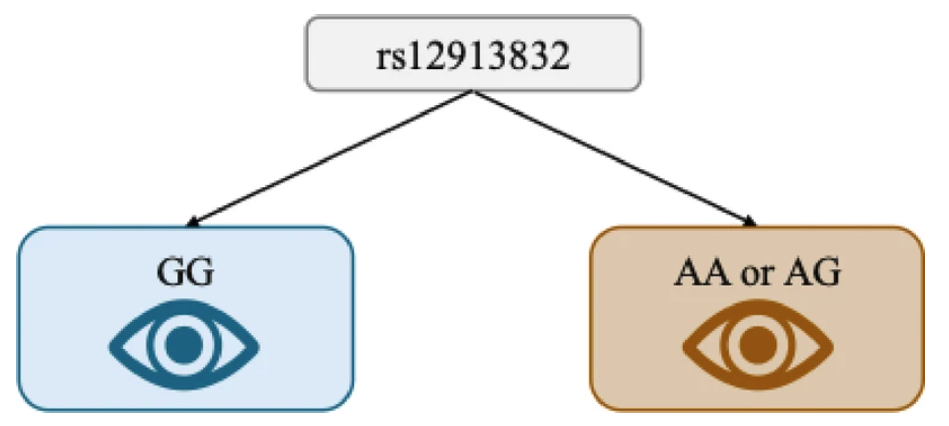
\includegraphics[width=0.95\textwidth, height=4cm, keepaspectratio]{img/diagrams/eye-color.png}%
        \captionof{figure}{Color de ojos esperado basado en el polimorfismo rs12913832 (\textit{HERC2}) en una población canadiense \parencite{abbatangelo2026-eye-color}.}%
      }%
      \only<2>{%
        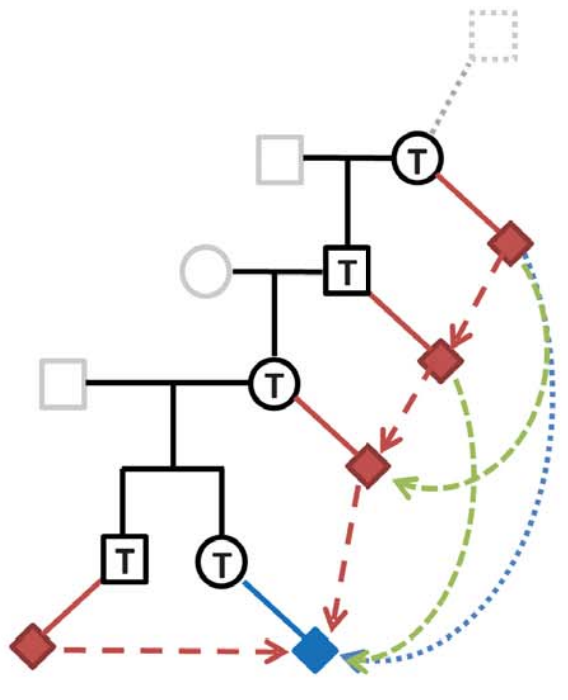
\includegraphics[width=0.95\textwidth, height=4cm, keepaspectratio]{img/diagrams/kong2018-ige.png}%
        % \captionof{figure}{Genetic nurture \parencite{kong2018-parental-genotype}.}%
        \captionof{figure}{Diagrama para el modelado de IGEs \parencite{kong2018-parental-genotype}.}%
      }%
      \only<3>{%
        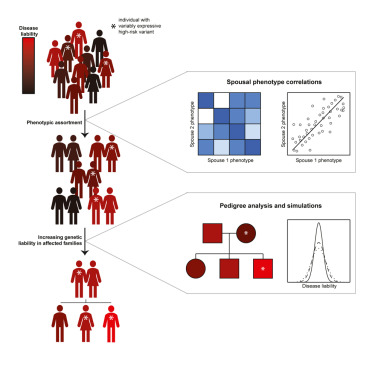
\includegraphics[width=0.95\textwidth, height=4cm, keepaspectratio]{img/diagrams/smolen2023-assortative-mating.jpg}%
        % \captionof{figure}{Assortative mating \parencite{smolen2023-assortative-mating}.}%
        \captionof{figure}{Fenotipos y genotipos (indirectamente) pueden estar correlacionados en la selección de parejas \parencite{smolen2023-assortative-mating}.}%
      }%
      \only<4>{%
        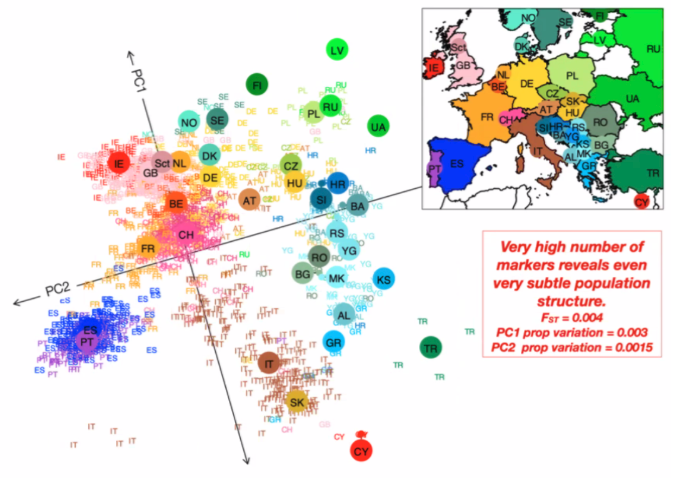
\includegraphics[width=0.95\textwidth, height=4cm, keepaspectratio]{img/diagrams/novembre2008-pca.png}%
        % \captionof{figure}{Population stratification \parencite{novembre2008-humanitiesandsocialsciences}.}%
        \captionof{figure}{Fenotipos y genotipos son segregados en regiones geográficas por barreras naturales, sociales o culturales \parencite{novembre2008-humanitiesandsocialsciences}.}%
      }%
    \end{column}
  \end{columns}
\end{frame}

% ============================================================
% Static TikZ: Genetic Effects Shrinkage
% ============================================================
\usetikzlibrary{decorations.pathreplacing, arrows.meta}

\begin{frame}{Sesgos en GWAS}
  \centering
  \vspace{0.5cm}
  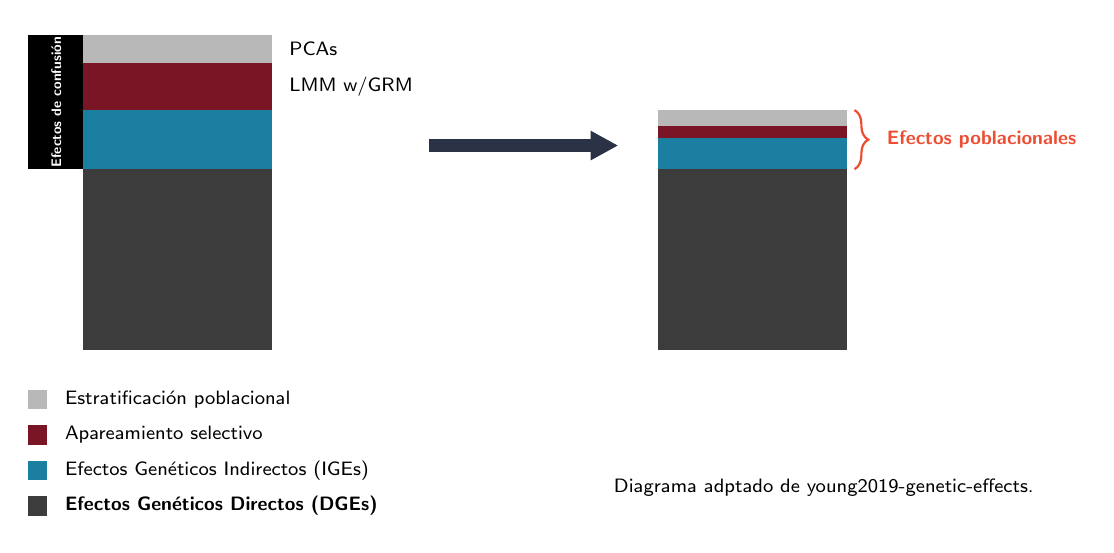
\begin{tikzpicture}[
    every node/.style={font=\sffamily},
  ]

    % --- Color definitions ---
    \definecolor{dgegray}{HTML}{3C3C3C}
    \definecolor{nurblue}{HTML}{1A7FA0}
    \definecolor{assred}{HTML}{7A1525}
    \definecolor{stratgray}{HTML}{B8B8B8}
    \definecolor{sideblack}{HTML}{000000}
    \definecolor{arrowdark}{HTML}{2B3245}
    \definecolor{bracered}{HTML}{ED4E33}

    % --- Dimensions for left bar (copied from previous slide) ---
    \def\barW{2.4}
    \def\barX{-0.5}
    \def\hdge{2.3}
    \def\hBlue{0.75}
    \def\hRed{0.6}
    \def\hGray{0.35}

    % --- Dimensions for right bar ---
    \def\barXRight{6.8}
    \def\hBlueR{0.4}
    \def\hRedR{0.15}
    \def\hGrayR{0.2}

    % --- LEFT BAR ---
    % DGE
    \fill[dgegray] (\barX, 0) rectangle (\barX+\barW, \hdge);
    % Crianza / IGEs
    \fill[nurblue] (\barX, \hdge) rectangle (\barX+\barW, \hdge+\hBlue);
    % Apareamiento / Assortative
    \fill[assred] (\barX, \hdge+\hBlue) rectangle (\barX+\barW, \hdge+\hBlue+\hRed);
    % Estratificación / Pop Strat
    \fill[stratgray] (\barX, \hdge+\hBlue+\hRed) rectangle (\barX+\barW, \hdge+\hBlue+\hRed+\hGray);

    % Sidebar "Confounding effects"
    \fill[sideblack] (\barX-0.7, \hdge) rectangle (\barX, \hdge+\hBlue+\hRed+\hGray);
    \node[rotate=90, anchor=mid, text=white, font=\sffamily\bfseries\tiny]
      at (\barX-0.35, \hdge + 0.5*\hBlue + 0.5*\hRed + 0.5*\hGray)
      % {Confounding effects};
      {Efectos de confusión};

    % Left bar annotations
    \node[anchor=west, font=\sffamily\scriptsize] at (\barX+\barW+0.1, \hdge+\hBlue+\hRed+0.5*\hGray) {PCAs};
    \node[anchor=west, font=\sffamily\scriptsize] at (\barX+\barW+0.1, \hdge+\hBlue+0.5*\hRed) {LMM w/GRM};

    % --- MIDDLE ARROW ---
    \draw[-{Triangle[width=10pt,length=10pt]}, line width=5pt, color=arrowdark] 
      (\barX+\barW+2.0, \hdge+0.3) -- (\barXRight-0.5, \hdge+0.3);

    % --- RIGHT BAR ---
    % DGE (same height)
    \fill[dgegray] (\barXRight, 0) rectangle (\barXRight+\barW, \hdge);
    % IGEs (shrunk)
    \fill[nurblue] (\barXRight, \hdge) rectangle (\barXRight+\barW, \hdge+\hBlueR);
    % Assortative (shrunk)
    \fill[assred] (\barXRight, \hdge+\hBlueR) rectangle (\barXRight+\barW, \hdge+\hBlueR+\hRedR);
    % Pop Strat (shrunk)
    \fill[stratgray] (\barXRight, \hdge+\hBlueR+\hRedR) rectangle (\barXRight+\barW, \hdge+\hBlueR+\hRedR+\hGrayR);

    % Curly brace and "Inflated results"
    \draw[bracered, thick, decorate, decoration={brace, amplitude=5pt, mirror}] 
      (\barXRight+\barW+0.1, \hdge) -- (\barXRight+\barW+0.1, \hdge+\hBlueR+\hRedR+\hGrayR) 
      node[midway, right=8pt, font=\sffamily\bfseries\scriptsize, text=bracered]
      % {Inflated results};
      {Efectos poblacionales};

    % --- LEGEND (Bottom Left) ---
    \def\legX{\barX-0.7}
    \def\legY{-0.5}
    \def\legSep{0.45}
    \def\legBoxW{0.25}
    \def\legBoxH{0.25}

    % Pop Strat
    \fill[stratgray] (\legX, \legY) rectangle +(\legBoxW, -\legBoxH);
    \node[anchor=west, font=\sffamily\scriptsize] at (\legX+\legBoxW+0.1, \legY-0.5*\legBoxH)
      % {Population stratification};
      {Estratificación poblacional};

    % Assortative Mating
    \fill[assred] (\legX, \legY-1*\legSep) rectangle +(\legBoxW, -\legBoxH);
    \node[anchor=west, font=\sffamily\scriptsize] at (\legX+\legBoxW+0.1, \legY-1*\legSep-0.5*\legBoxH)
      % {Assortative mating};
      {Apareamiento selectivo};

    % IGEs
    \fill[nurblue] (\legX, \legY-2*\legSep) rectangle +(\legBoxW, -\legBoxH);
    \node[anchor=west, font=\sffamily\scriptsize] at (\legX+\legBoxW+0.1, \legY-2*\legSep-0.5*\legBoxH)
      % {Indirect Genetic Effects (IGEs)};
      {Efectos Genéticos Indirectos (IGEs)};

    % DGEs
    \fill[dgegray] (\legX, \legY-3*\legSep) rectangle +(\legBoxW, -\legBoxH);
    \node[anchor=west, font=\sffamily\bfseries\scriptsize] at (\legX+\legBoxW+0.1, \legY-3*\legSep-0.5*\legBoxH)
      % {Direct Genetic Efects (DGEs)};
      {Efectos Genéticos Directos (DGEs)};

    % --- CITATION (Bottom Right) ---
    \node[anchor=south east, font=\sffamily\scriptsize] 
      at (\barXRight+\barW+2.5, \legY-3*\legSep-0.5*\legBoxH) 
      % {Adapted from \textcite{young2019-genetic-effects}.};
      {Diagrama adptado de \textcite{young2019-genetic-effects}.};

  \end{tikzpicture}
\end{frame}

% ============================================================
% Family-based GWAS Limitations
% ============================================================
\begin{frame}[c]{Family-based GWAS}
  \begin{columns}[c]

    % --- LEFT COLUMN: Image ---
    \begin{column}{0.55\textwidth}
      \centering
      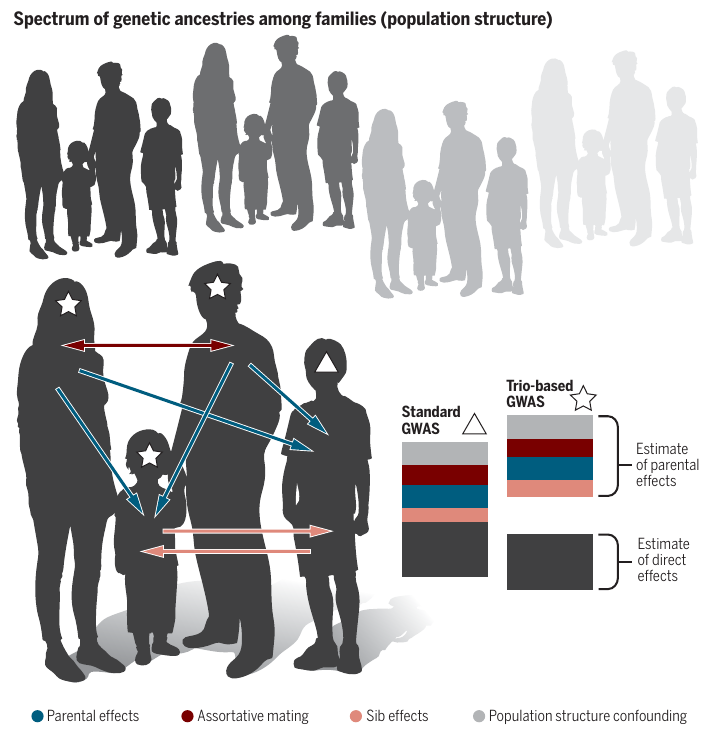
\includegraphics[height=5.15cm, keepaspectratio]{img/diagrams/young2019-signals-captured-gwas.png}
      % \captionof{figure}{Signals captured by GWAS of related individuals and families \parencite{young2019-genetic-effects}.}
      \captionof{figure}{Señales capturadas por un GWAS de individuos relacionados y familias. Recuperado de \textcite{young2019-genetic-effects}.}
    \end{column}

    % --- RIGHT COLUMN: Text ---
    \begin{column}{0.45\textwidth}

      % --- Spanish ---
      {Los FGWAS pueden discriminar entre DGEs y Efectos Poblacionales} \\[1pt]
      {\tiny \parencite{visscher2006-populationgenetics,young2019-genetic-effects}}\\[1em]
      \pause
      \centering
      {\bfseries\large\color[HTML]{7CBB00}
        PERO
      }\\[0.5em]
      \begin{columns}[T]
        \small
        \begin{column}{0.425\textwidth}
          {Evidencia de una señal biológica \textbf{verdadera}}
        \end{column}
        \begin{column}{0.05\textwidth}
          vs.
        \end{column}
        \begin{column}{0.425\textwidth}
          {Limitado a solamente individuos con \textbf{ambos padres genotipados}}
        \end{column}
      \end{columns}
      \pause
      \vspace{3em}
      {\centering\large
        Recuperar poder estadístico es \textbf{prioridad}
      }
    \end{column}
  \end{columns}
\end{frame}

% ============================================================
% Why use the MCPS?
% ============================================================
 \begin{frame}[c]{Estudio Prospectivo de la Ciudad de México (MCPS)}
  \begin{columns}[T]
    % --- COLUMN A ---
    \begin{column}{0.35\textwidth}
      \centering
      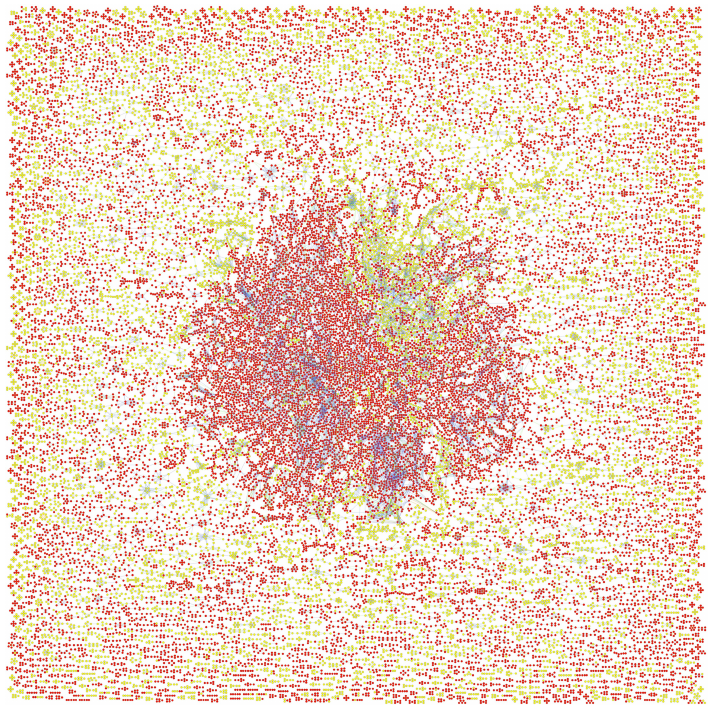
\includegraphics[height=3cm]{img/diagrams/mcps-family-network.png}\\[0.5em]
      {\bfseries
        Redes familiares densas
      }\\[3pt]
      {\tiny
        MCPS \parencite{ziyatdinov2023-mcps} proporciona más del \textit{doble} de pares de familiares de primer grado que UK Biobank \parencite{bycroft2018-ukbiobank} \\[2pt]
      }
    \end{column}
    % --- COLUMN B ---
    \begin{column}{0.65\textwidth}
      \centering
      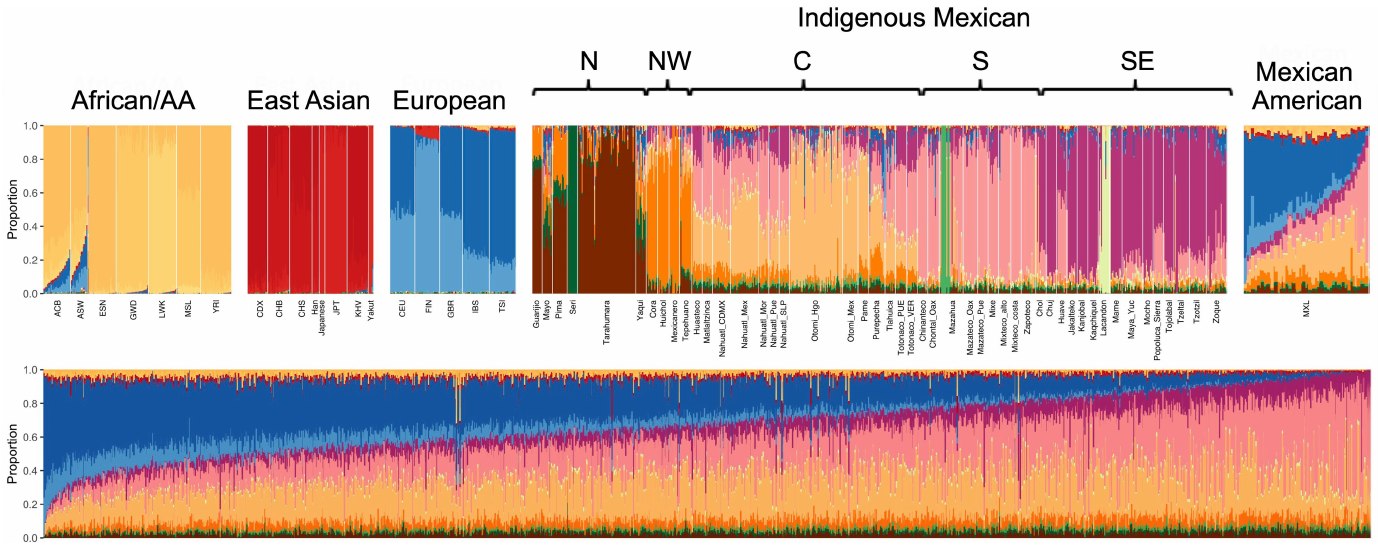
\includegraphics[height=3cm]{img/diagrams/mcps-admixture.png}\\[0.5em]
      {\bfseries
        Mestizaje reciente
      }\\[3pt]
      {\tiny
        Ancestrías provenientes de Europa y África, e indígenas de México.
        Mejorar representación en estudios genómicos \parencite{popejoy2016-admixture,martin2017-pgs}.
      }
    \end{column}
  \end{columns}
  \centering
  \vspace{2em}
  {\small
    \textcite{tapia-conyer2006-mcps,ziyatdinov2023-mcps}
  }
\end{frame}